%This is part of Un soupçon de mathématique sans être agressif pour autant
% Copyright (c) 2012
%   Laurent Claessens, Pauline Klein
% See the file fdl-1.3.txt for copying conditions.

%+++++++++++++++++++++++++++++++++++++++++++++++++++++++++++++++++++++++++++++++++++++++++++++++++++++++++++++++++++++++++++
\section{Introduction, domaine de définition}
%+++++++++++++++++++++++++++++++++++++++++++++++++++++++++++++++++++++++++++++++++++++++++++++++++++++++++++++++++++++++++++


\begin{example} \label{ExemVmCkIH}
    Un petit tour de magie. Choisissez un nombre entre \( 1\) et \( 10\). Ajoutez \( 5\), multipliez par \( 2\), ajoutez \( 7\), enlevez le double du nombre de départ.

    Le nombre que vous avez maintenant est \( 17\).
\end{example}

\begin{definition}
    Soit \( \defD\) un ensemble de nombres. On définit une \defe{fonction}{fonction} \( f\) sur \( \defD\) en associant à chaque nombre \( x\) dans \( \defD\) un seul nombre \( y\). Dans ce cas nous disons que \( f\) est une fonction de la \defe{variable}{variable} \( x\).
\end{definition}

La partie difficile de cette définition est l'introduction du domaine de définition \( \defD\). Oublions la un instant pour comprendre le reste. Sans parler de \( \defD\), la définition s'écrit :

\begin{quote}
    On définit une \defe{fonction}{fonction} \( f\) en associant à chaque nombre \( x\) un seul nombre \( y\).
\end{quote}
Cela n'est rien d'autre qu'une façon savante de dire qu'une fonction «prend un nombre en entrée, fait des calculs et retourne un nombre en sortie».

Pourquoi introduit-t-on le domaine de définition ? Simplement parce que toute fonction ne va pas accepter toutes les valeurs en entrée. Le domaine de définition est l'ensemble des valeurs acceptées.

\begin{example}
    Soit la fonction qui à la longueur d'un segment fait correspondre la surface du carré construit sur ce segment. Cette fonction n'est définie que sur les nombres positifs (parce qu'il n'existe pas de segments de longueurs négatives). Nous écrivons donc
    \begin{equation}
        \begin{aligned}
            f\colon \mathopen[ 0 , \infty [&\to \eR \\
            x&\mapsto x^2,
        \end{aligned}
    \end{equation}
    et nous avons \( f(x)=x^2\).
\end{example}

\begin{example}
    Soit la fonction qui a un nombre entier fait correspondre la somme de ses chiffres. Par exemple \( f(0)=0\) et \( f(123)=6\). Cette fonction est définie sur les entiers et retourne un entier. Nous pouvons écrire
    \begin{equation}
        \begin{aligned}
            f\colon \eN&\to \eN \\
            x&\mapsto f(x). 
        \end{aligned}
    \end{equation}
    Ici il est compliqué de donner une forme explicite pour \( f\).
\end{example}


En ce qui concerne les notations, nous écrivons
\begin{equation}
    \begin{aligned}
        f\colon \defD&\to \eR \\
        x&\mapsto f(x). 
    \end{aligned}
\end{equation}
Cela signifie que \( \defD\) est l'\defe{ensemble de définition de \( f\)}{ensemble!de définition}, c'est à dire l'ensemble des nombres sur lesquels \( f\) peut être appliquée. Le symbole \( \eR\) désigne l'ensemble de tous les nombres.

%+++++++++++++++++++++++++++++++++++++++++++++++++++++++++++++++++++++++++++++++++++++++++++++++++++++++++++++++++++++++++++
\section{Intermède : pourquoi on ne peut pas diviser par zéro ?}
%+++++++++++++++++++++++++++++++++++++++++++++++++++++++++++++++++++++++++++++++++++++++++++++++++++++++++++++++++++++++++++

La fraction \( \frac{1}{ 0.1 }\) est le nombre de fois que \( 0.1\) rentre dans \( 1\). Cela vaut \( 10\) parce qu'il faut \( 10\) soit \( 0.1\) pour faire \( 1\).

Que vaut \( \frac{1}{ 0.0001 }\) ? C'est le nombre de fois que \( 0.0001\) rentre dans \( 1\), c'est à dire dix mille.

Que vau{\bf rait} \( \frac{1}{ 0 }\) ? C'est le nombre de fois qu'il faut prendre zéro pour obtenir \( 1\).

\begin{example}
    Considérons la fonction qui a un nombre fait correspondre son inverse : \( f(x)=\frac{1}{ x }\). Pour se dérouiller le cerveau, je propose quelque valeurs :
    \begin{equation}
        \begin{aligned}[]
            f(1)&=1&f(5)&=\frac{1}{ 5 }&f(\frac{ 2 }{ 3 })=\frac{ 3 }{ 2 }\\
            f(\frac{ 1 }{ 4 })&=4&f(-3)&=-\frac{1}{ 3 }&f(-1)&=-1.
        \end{aligned}
    \end{equation}
    Cette fonction est implémentée en python de la façon suivante :

\lstinputlisting{ex_inverse.py}

donne

\lstinputlisting[title=Résultat]{res_ex_inverse.txt}

Très clairement, python ne veut pas calculer l'inverse de zéro et plante sur un message on ne peut plus clair : \info{ZeroDivisionError: division by zero}.

Effectivement, l'inverse de zéro n'existe pas. Le domaine de notre fonction \( f(x)=1/x\) n'est donc pas \( \eR\) tout entier, mais seulement \( \eR\setminus\{ 0 \}\).

\end{example}

\begin{Aretenir}        \label{ArtJgipNt}
    Il n'est pas permis de diviser par zéro. Une fonction qui contient un dénominateur ne peut pas avoir dans son domaine de définition des \( x\) qui annulent le dénominateur. Autrement dit dès que vous voyez
    \begin{equation}
        \frac{1}{ f(x) }
    \end{equation}
    vous devez résoudre l'équation \( f(x)=0\).
\end{Aretenir}

%+++++++++++++++++++++++++++++++++++++++++++++++++++++++++++++++++++++++++++++++++++++++++++++++++++++++++++++++++++++++++++
\section{Antécédent}
%+++++++++++++++++++++++++++++++++++++++++++++++++++++++++++++++++++++++++++++++++++++++++++++++++++++++++++++++++++++++++++

\begin{Aretenir}
Une fonction associe à chaque nombre de l'ensemble de définition \emph{un seul} nombre, appelé \defe{image}{image}. Si \( a\) est un nombre, un \defe{antécédent}{antécédent} de \( a\) par la fonction \( f\) est un nombre \( x\in\defD\) tel que 
\begin{equation}
    f(x)=a.
\end{equation}
Autrement dit, les antécédents de \( a\) sont les éléments de \( \eR\) dont l'image par \( f\) est \( a\).

Il peut arriver qu'un nombre ait plusieurs antécédents.
\end{Aretenir}


\begin{example}
    Pour la fonction \( f(x)=2x-1\), un antécédent de \( 5\) est le nombre \( 3\). Un antécédent du nombre \( -10\) est la nombre \( -9/2\).
\end{example}

\begin{Aretenir}
    Trouver les antécédents de \( a\) par la fonction \( f\) revient à trouver les solutions de l'équation
    \begin{equation}
        f(x)=a.
    \end{equation}
\end{Aretenir}


\begin{example}

    Les antécédents de \( 4\) pur la fonction \( f(x)=2x-1\) sont les solutions de l'équation
    \begin{equation}
        2x-1=4
    \end{equation}
    c'est à dire \( x=\frac{ 5 }{2}\). Il se fait qu'il y en a un seul.

    Plus généralement l'antécédent de \( a\) pour cette fonction est la solution de l'équation
    \begin{equation}
        2x-1=a,
    \end{equation}
    c'est à dire le nombre \( x=\frac{ a+1 }{ 2 }\).
\end{example}

\begin{example} \label{EqlaIGDz}
    Si nous avons une série statistique de \( n\) valeurs, pour trouver le premier quartile nous devons diviser \( n\) par \( 4\) et prendre l'entier le plus proche vers le haut. Cela donne le numéro de la valeur correspondante au premier quartile.

    En python, la fonction qui donne le numéro de la valeur du premier quartile en fonction de \( n\) est
    \begin{quote}
        \info{math.ceil(n/4)}
    \end{quote}
    Notons \( f\) cette fonction. Son domaine est l'ensemble des entiers non nuls. Le graphique de cette fonction est donné à la figure \ref{LabelFigMathCeilwCXIJZ}.
\newcommand{\CaptionFigMathCeilwCXIJZ}{Le numéro de la valeur du premier quartile en fonction du nombre de valeurs.}
\input{Fig_MathCeilwCXIJZ.pstricks}

    Le graphique est uniquement constitué de points. Pas de lignes entre, parce qu'il n'existe pas de séries statistiques comprenant \( 3.7\) valeurs par exemple. 
\end{example}

\Exo{Seconde-0053}

\begin{example}
    Soit la fonction définie sur \( \defD=\{ -5,-1,1,3,9 \}\) de la façon suivante :
    \begin{equation}
        \begin{array}[h]{|c||c|c|c|c|c|c|}
            \hline
            x&-5&-1&1&3&9&10\\
            \hline
            f(x)&0&2&-3&7&2&5\\
            \hline
        \end{array}
    \end{equation}
    Nous pouvons dire que
    \begin{enumerate}
        \item
            L'image de \( 1\) par \( f\) est \( -3\).
        \item
            L'unique antécédent de \( 7\) est \( 3\).
        \item
            Les nombres \( -1\) et \( 9\) sont tous deux des antécédents de \( 2\).
    \end{enumerate}
\end{example}

\begin{example}
    Soit la fonction \( f(x)=(x+1)^2\). Nous avons \( f(-1)=0\), \( f(4)=25\); nous disons que \( 0\) est l'image de \( -1\) par \( f\) et que \( 25\) est l'image de \( 4\) par \( f\).

    Remarquons que \( f(-2)=1\) et \( f(0)=1\). Donc \( -2\) et \( 0\) sont deux antécédents de \( 1\).
\end{example}

\begin{example}
    Le nombre \( 4\) est un antécédent de \( 3\) pour la fonction \( f(x)=\frac{ x }{ 2 }+1\).
\end{example}

\begin{example}
    Les nombres \( 3\) et \( -3\) sont tout deux des antécédents de \( 9\) pour la fonction \( x\mapsto x^2\).
\end{example}

%+++++++++++++++++++++++++++++++++++++++++++++++++++++++++++++++++++++++++++++++++++++++++++++++++++++++++++++++++++++++++++
\section{Modélisation par une fonction}
%+++++++++++++++++++++++++++++++++++++++++++++++++++++++++++++++++++++++++++++++++++++++++++++++++++++++++++++++++++++++++++

Les exemples de fonctions dans la «vraie» vie sont nombreux.

\begin{example}
    Soit un triangle rectangle isocèle dont les côtés de l'angle droit sont de longueur \( x\). Alors la surface est donnée par la fonction
    \begin{equation}
        f(x)=\frac{ x^2 }{2}.
    \end{equation}
    Le domaine est \( \defD=\mathopen] 0 , \infty \mathclose[\) parce que \( x\) représente une longueur.
\end{example}

\begin{example}
    Un vélo se déplace à \( \unit{20}{\kilo\meter\per\hour}\). Après un temps \( t\), il aura parcouru une distance
    \begin{equation}
        d(t)=20t
    \end{equation}
    kilomètres. Ici le domaine est plus délicat; il dépend du contexte.

    Notons que la variable d'une fonction n'est pas obligatoirement toujours notée \( x\) et que la fonction n'est pas toujours obligatoirement notée \( f\).
\end{example}

\begin{example}
    Vous verrez dans un cours de physique que si on lance un objet verticalement avec une vitesse initiale \( v_0\), alors la hauteur en fonction du temps est donnée par
    \begin{equation}
        h(t)=v_0t-\frac{ gt^2 }{2}
    \end{equation}
    où \( g\) est l'accélération de la gravitation sur Terre (environ \( \unit{10}{\meter\per\second\squared}\)).
\end{example}

%+++++++++++++++++++++++++++++++++++++++++++++++++++++++++++++++++++++++++++++++++++++++++++++++++++++++++++++++++++++++++++
\section{Courbe représentative d'une fonction}
%+++++++++++++++++++++++++++++++++++++++++++++++++++++++++++++++++++++++++++++++++++++++++++++++++++++++++++++++++++++++++++

%TODO : il faut essayer de refaire une figure pour tous les dessins de Pauline.
Soit $f$ une fonction définie sur un ensemble $\defD$.

\begin{definition}
    On appelle \defe{représentation graphique}{représentation graphique (d'une fonction)}, ou le \defe{graphe}{graphe} de $f$, l'ensemble des points $(x,y)$ tels que $x\in\defD$ et $y=f(x)$.
\end{definition}

\newcommand{\CaptionFigExFonction}{Comment tracer la fonction \( f(x)=2x+1\) ?}
\input{Fig_ExFonction.pstricks}

Nous donnons à la figure \ref{LabelFigExFonction} le tracé de la fonction \( f(x)=2x+1\). La figure \ref{LabelFigExFonctionssLabelSubFigExFonction0} donne quelque points du graphe de la fonction. La figure \ref{LabelFigExFonctionssLabelSubFigExFonction1} donne le graphe complet de la fonction. Comment le construit-on ? Par définition pour chaque \( x\) sur l'axe des abscisses (il y en a une infinité), il faut calculer le nombre \( f(x)\) et mettre dans le plan le point de coordonnées \( \big( x,f(x) \big)\).

En pratique, il n'est pas possible de calculer \( f(x)\) pour \emph{tous} les \( x\) réels\footnote{Chuck Norris peut le faire.}. C'est pourquoi nous nous contentons qu'en calculer quelque uns, et nous les relions «le plus intelligemment possible».

\begin{example}
    Soit la fonction \( f(x)=3x-1\).
    \begin{enumerate}
        \item
            Le point \( (0;-1)\) est sur la courbe représentative de \( f\) parce que \( f(0)=1\).
        \item
            Le point \( (10;29)\) est également sur la courbe parce que \( f(10)=29\).
        \item
            Le point \( (2;3)\) n'est par contre pas sur le graphe parce que \( f(2)=5\neq 4\).
    \end{enumerate}
\end{example}

Quelque conseils pour dessiner.
\begin{itemize}
    \item
        Pour une valeur $x$ sur l'axe des abscisses, il y a un et un seul point d'abscisse $x$ sur la courbe.
    \item
        Pour tracer une courbe, il faut placer des points. Plus on choisit de points, plus la courbe sera précise.
    \item
        Si possible, trouver quelque valeurs clefs. Par exemple on cherchera les points d'intersection entre les axes et les courbe. Le point \( (0,f(0)) \) est intéressant à mettre, ainsi que les points \( x\) tels que \( f(x)=0\).
\end{itemize}

\begin{example}
    Créons un petit programme définissant la fonction \( f(x)=x^2-2\) et en calculant \( 10\) valeurs régulièrement espacées entre \( -5\) et \( 5\). La production d'une liste de nombre régulièrement espacés est un travail pour la fonction \info{numpy.linspace}. La syntaxe en est 
\begin{quote}
    \info{numpy.linspace(a,b,num=n)}
\end{quote}
Cela est une liste de \info{n} nombres régulièrement espacés entre \info{a} et \info{b}. En ce qui concerne le carré, en python les puissances sont données par \info{**}. Par exemple \info{a**3} est le cube de \info{a} :
\begin{verbatim}
>>> 2**3
8
\end{verbatim}
Le programme est

\lstinputlisting{ex_graphe.py}

Le programme donne :

\lstinputlisting[title=Résultat]{res_ex_graphe.txt}
    
\end{example}

%---------------------------------------------------------------------------------------------------------------------------
\subsection{Fonctions linéaires et affines}
%---------------------------------------------------------------------------------------------------------------------------

\begin{definition}
    Une classe importante de fonctions sont les fonctions de la forme \( f(x)=ax\) où \( a\) est un nombre. Une telle fonction est dite \defe{linéaire}{linéaire (fonction)}. 

    Les fonctions du type \( f(x)=ax+b\) sont des fonctions \defe{affines}{affine (fonction)}. 
\end{definition}


\begin{Aretenir}
    Les fonctions linéaires et affines sont très importantes parce que leur graphe sont des droites. 
    \begin{itemize}
        \item 
    Les fonctions linéaires sont des droites qui passent par l'origine \( (0;0)\).
    \item
    Les fonctions affines (avec \( b\neq 0\)) sont des droites ne passant pas par \( (0;0)\).
    \end{itemize}
\end{Aretenir}
Si $f$ est une fonction affine définie pour $x\in\eR$ par $f(x)=ax+b$ alors l'équation de la droite représentative de la fonction est $y=ax+b$. 

Pour tracer le graphe d'une fonction affine.
\begin{itemize}
    \item
        Vu que le graphe est une droite, il suffit de deux points.
    \item
        Les fonction linéaires passent par l'origine \( (0;0)\).
    \item 
        Pour un tracé à la règle, il est plus précis de prendre deux points relativement éloignés.
    \item
        La droite \( f(x)=ax+b\) monte si \( a>0\) et descend si \( a<0\). La pente est d'autant plus raide que \( a\) est grand.
\end{itemize}

Quelque exemples à la figure \ref{LabelFigGrapheAffinHqXJGx}.
\newcommand{\CaptionFigGrapheAffinHqXJGx}{Des graphes de fonctions linéaires et affines.}
\input{Fig_GrapheAffinHqXJGx.pstricks}

%---------------------------------------------------------------------------------------------------------------------------
\subsection{Ce qui n'est pas une fonction}
%---------------------------------------------------------------------------------------------------------------------------

%    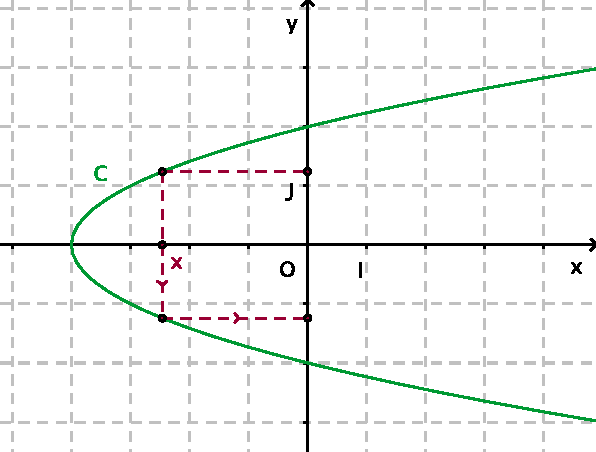
\includegraphics[width=5cm]{F_NonFct.pdf}

\begin{multicols}{2}
    Cette courbe ne représente pas une fonction, car à partir de \( x=-4\), les nombres ont deux images. Les courbes données par des fonctions sont des courbes acceptant une seule ordonnée pour chaque abscisse.

\columnbreak

%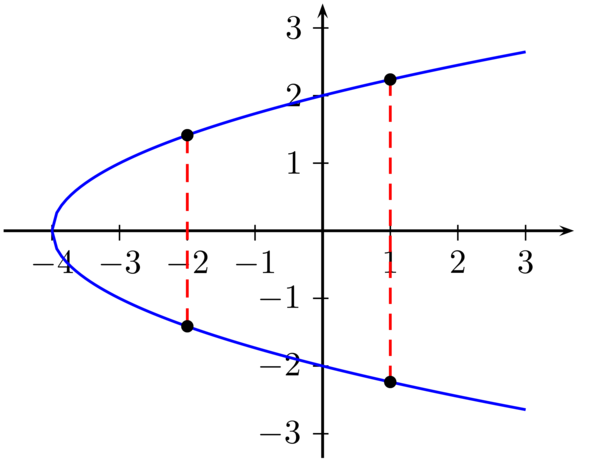
\includegraphics{Picture_FIGLabelFigPasFonctionYoQfSuPICTPasFonctionYoQfSu-for_eps.pdf}

\input{Fig_PasFonctionYoQfSu.pstricks}

\end{multicols}

%---------------------------------------------------------------------------------------------------------------------------
\section{Résolution graphique d'(in)équations} 
%---------------------------------------------------------------------------------------------------------------------------

\subsection{Lecture graphique des images et des antécédents}

\begin{multicols}{2}

    Nous considérons la fonction
    \begin{equation}
        \begin{aligned}
            f\colon \eR&\to \eR \\
            x&\mapsto x^2 
        \end{aligned}
    \end{equation}
    dont le graphe est donné ci-contre. À chaque réel $x$, nous associons l'abscisse $y=f(x)$.  À l'aide du graphe donné, répondre aux questions suivantes.

    \begin{itemize}
        \item Image de $1,5$ ? 
        \item Antécédent de $3,5$ ?  
        \item Antécédent de $-1$ ? 
        \item Antécédent de $0$ ? 
    \end{itemize}

    \columnbreak

    %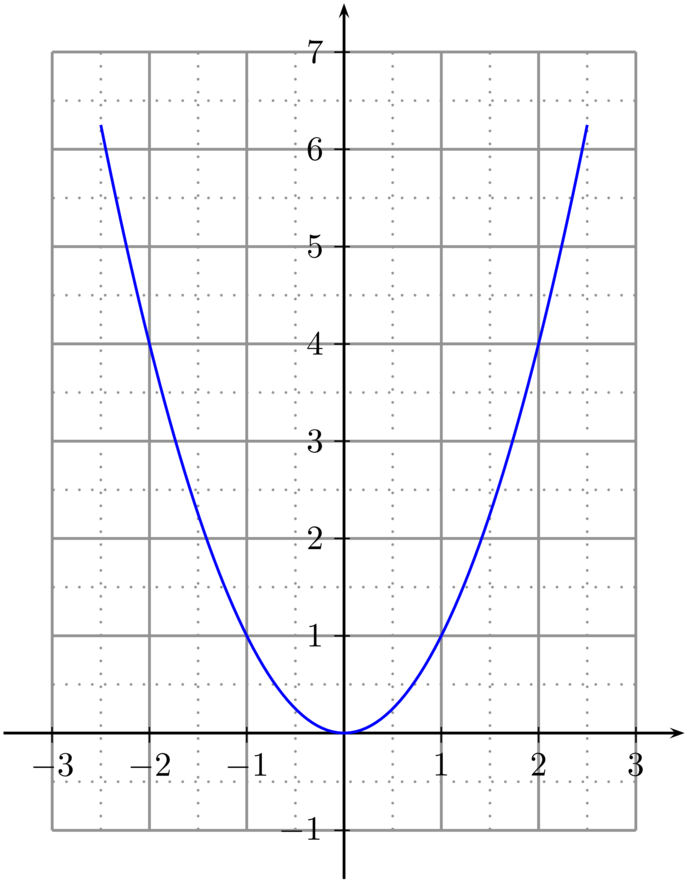
\includegraphics{Picture_FIGLabelFigFCarreQFhsWzPICTFCarreQFhsWz-for_eps.pdf}
    %\newcommand{\CaptionFigFCarreQFhsWz}{Le graphe de la fonction \( x\mapsto x^2\).}
    \input{Fig_FCarreQFhsWz.pstricks}

\end{multicols}

  \begin{example}
Compléter le tableau suivant pour la fonction $f(x)=x^2$.
\begin{equation}
\begin{array}[h]{|c|c|c|c|c|c|c|c|c|c|c|c|}
  \hline  
  x & -4 & -3 & -2 & -1 & 0 & 1 & 2 & 3 & 4 & -0,5 & 0,5  \\
  \hline
  y & 16 &&&&&&&&&&0.25\\
  \hline
\end{array}
\end{equation}
  \end{example}


\subsection{Résolution graphique d'équations}

\begin{Aretenir}
    Soit $k$, un réel fixé. Résoudre l'équation $f(x)=k$ revient à chercher les antécédents par $f$ du nombre $k$.

Le nombre de solutions de l'équation $f(x)=k$ est égal au nombre de points d'intersection de la courbe représentative de \( f\) avec la droite $d$ d'équation $y=k$. Les solutions sont les abscisses de ces points d'intersection. 
\end{Aretenir}


\begin{example}
    \begin{multicols}{2}
  Nous cherchons à résoudre $f(x)=4$. 
  \begin{itemize}
      \item 
          Nous traçons la droite horizontale d'équation \( y=4\);
      \item
          nous observons les points d'intersection de cette droite avec la courbe;
      \item
          les solutions de l'équation sont les abscisses de ces points.
  \end{itemize}

\columnbreak


%The result is on figure \ref{LabelFigExCarrexvfvre}. % From file ExCarrexvfvre
%\newcommand{\CaptionFigExCarrexvfvre}{<+Type your caption here+>}
\input{Fig_ExCarrexvfvre.pstricks}

    \end{multicols}

    Sans surprises, les solutions de \( x^2=4\) sont \( x=2\) et \( x=-2\).

\end{example}

\begin{Aretenir}
    Résoudre l'équation $f(x)=g(x)$ revient à déterminer les abscisses des points d'intersection des courbes représentatives de \( f\) et \( g\).
\end{Aretenir}


\begin{multicols}{2}

    Les solutions de l'équation \( f(x)=g(x)\) sont les abscisses des points d'intersection des deux courbes. Pour les trouver, il suffit de repérer les points d'intersections, puis de les projeter sur l'axe horizontal.

    Dans le cas de la figure ci-contre, les solutions sont approximativement \( x=-3.6\), \( x=-1.1\) et \( x=1.5\).

\columnbreak

%The result is on figure \ref{LabelFigExEquationIntersectioniSHPTw}. % From file ExEquationIntersectioniSHPTw
%\newcommand{\CaptionFigExEquationIntersectioniSHPTw}{<+Type your caption here+>}
\input{Fig_ExEquationIntersectioniSHPTw.pstricks}

\end{multicols}


\subsection{Résolution graphique d'inéquations}


%///////////////////////////////////////////////////////////////////////////////////////////////////////////////////////////
\subsubsection{Inéquation du type $f(x)<k$}
%///////////////////////////////////////////////////////////////////////////////////////////////////////////////////////////

\begin{Aretenir}
Les solutions de l'inéquation $f(x)<k$ sont les abscisses des points de $\mathscr{C}$ situés en-dessous de la droite d'équation $y=k$.

En particulier, les solutions de l'inéquation $f(x)<0$ sont les abscisses des points de la courbe représentative de \( f\) situés en-dessous de l'axe des abscisses, c'est-à-dire ayant une ordonnée strictement négative.
\end{Aretenir}

\begin{multicols}{2}
    Sur la figure ci-contre, nous résolvons \( f(x)\leq 2\). La procédure à suivre est la suivante.
    \begin{enumerate}
        \item
            Tracer la droite horizontale \( y=2\).
        \item
            Trouver les points d'intersection avec le graphe de \( f\).
        \item
            Les solutions sont les abscisses pour lesquelles le graphe de \( f\) est au-dessus du graphe de la droite \( y=2\).
    \end{enumerate}

    \columnbreak

%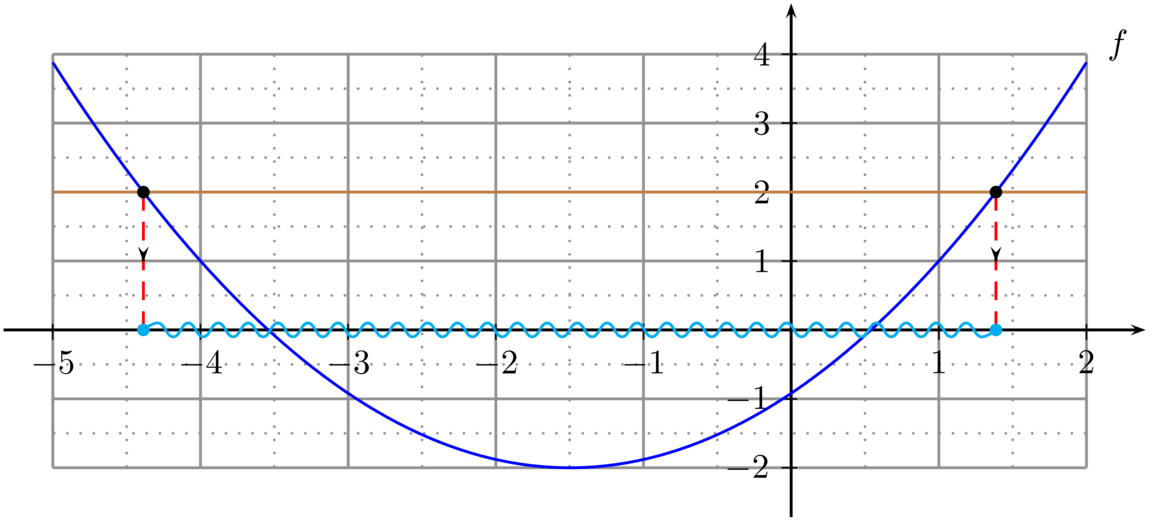
\includegraphics{Picture_FIGLabelFigExIneqOcAWMqPICTExIneqOcAWMq-for_eps.pdf}
    %\newcommand{\CaptionFigExIneqOcAWMq}{Les solutions de l'équation \( f(x)\leq 2\) sont en ondulé.}
    \input{Fig_ExIneqOcAWMq.pstricks}

\end{multicols}


\begin{remark}
    Ici nous avons résolut l'équation \( f(x)\leq 2\). Les deux points extrêmes dont partie de l'ensemble des solutions. Si nous avions résolu \( f(x)<2\), alors les points extrêmes n'auraient pas fait partie de l'ensemble des solutions.
\end{remark}

On procède de la même manière pour les inégalités du type $f(x)>k$, $f(x)\geq k$, $f(x)\leq k$. 

%///////////////////////////////////////////////////////////////////////////////////////////////////////////////////////////
\subsubsection{Inéquation du type $f(x)<g(x)$}
%///////////////////////////////////////////////////////////////////////////////////////////////////////////////////////////

Les solutions de l'inéquation $f(x)<g(x)$ sont les abscisses des points pour lesquels la courbe de \( f\) est en-dessous de la courbe de \( g\).


\newcommand{\CaptionFigExIneqfgZWStde}{En cyan, l'ensemble des solutions de l'inéquation \( f(x)<g(x)\).}
\input{Fig_ExIneqfgZWStde.pstricks}

La figure \ref{LabelFigExIneqfgZWStde} montre la résolution d'une telle inéquation. Notons que l'ensemble des solutions peut être en plusieurs morceaux.


\section{Sens de variation d'une fonction}

\subsection{Notion intuitive}

\begin{multicols}{2}

    La fonction ci-contre descend jusqu'à \( -2.5\) puis monte entre \( -2.5\) et \( 2\) pour ensuite descendre.

    Nous disons qu'elle est
    \begin{itemize}
        \item 
            \emph{décroissante} sur \( \mathopen] \infty , -2.5 \mathclose]\);
        \item
            \emph{croissante} sur \( \mathopen[ -2.5 , 2 \mathclose]\);
        \item
            à nouveau décroissante sur \( \mathopen[ 2 , \infty [\).
    \end{itemize}
    
    \columnbreak

%    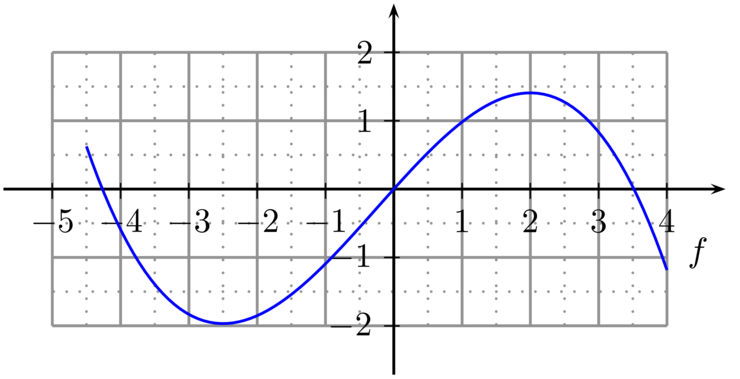
\includegraphics{Picture_FIGLabelFigExVariationRXTkocPICTExVariationRXTkoc-for_eps.pdf}
%The result is on figure \ref{LabelFigExVariationRXTkoc}.
%\newcommand{\CaptionFigExVariationRXTkoc}{<+Type your caption here+>}
\input{Fig_ExVariationRXTkoc.pstricks}

\end{multicols}


\subsection{Définition}

\begin{definition}
      Soit $f$ une fonction définie sur $\defD$ et $I$ un
      intervalle de $\defD$.\\[-2ex]
      \begin{enumerate}
          \item On dit que $f$ est \defe{croissante}{croissante (fonction)} sur $I$
        si et seulement si pour tous réels $a$ et $b$ de $I$, 
        si $a\leq b$ \ alors \ $f(a)\leq f(b)$.
    \item On dit que $f$ est \defe{décroissante}{décroissante (fonction)} sur $I$
        si et seulement si pour tous réels $a$ et $b$ de $I$, 
        si $a\leq b$ \ alors \ $f(a)\geq f(b)$. 
      \end{enumerate}
\end{definition}


\begin{remark}
    Une fonction croissante range les images dans le même ordre que les antécédents. Une fonction décroissante inverse cet ordre. 
\end{remark}


\begin{definition}
    On dit que $f$ est \defe{strictement croissante}{strictement croissante} sur~$I$
  si pour tous réels $a$ et $b$ de $I$ tels que $a<b$, on a $f(a)<f(b)$.

  La fonction \( f\) est \defe{strictement décroissante}{strictement décroissante} sur \( I\) si pour tous réels $a$ et $b$ de $I$ tels que $a<b$, on a $f(a)>f(b)$.
\end{definition}
La différence entre la croissance et la \emph{stricte} croissance est que l'inégalité est stricte.

\begin{definition}
    Soit \( I\) un intervalle de \( \eR\). Nous disons que la fonction \( f\) est \defe{monotone}{monotone} sur $I$ si elle est soit croissante sur $I$, soit décroissante sur $I$.
\end{definition}

\begin{multicols}{2}

    La fonction dessinée ci-contre n'est pas monotone sur l'intervalle \( \mathopen[ -2 , 0 \mathclose]\). Elle est
    \begin{itemize}
        \item 
            monotone décroissante sur \( \mathopen[ -2.5 , -1 \mathclose]\);
        \item
            monotone croissante sur \( \mathopen[ -1 , 1 \mathclose]\);
        \item
            monotone décroissante sur \( \mathopen[ 1 , 1.5 \mathclose]\).
    \end{itemize}

\columnbreak

%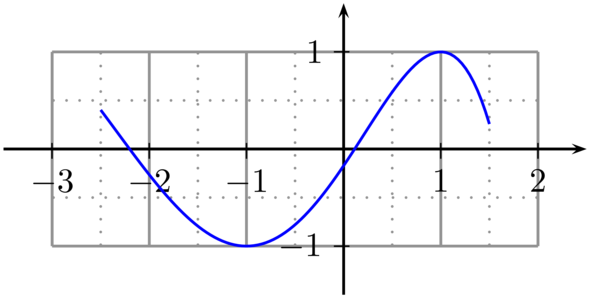
\includegraphics{Picture_FIGLabelFigGrapheVarndvdQMPICTGrapheVarndvdQM-for_eps.pdf}
%The result is on figure \ref{LabelFigGrapheVarndvdQM}.
%\newcommand{\CaptionFigGrapheVarndvdQM}{<+Type your caption here+>}
\input{Fig_GrapheVarndvdQM.pstricks}

\end{multicols}




\begin{definition}
    Soit \( I\) un intervalle. On dit que $f$ est \defe{constante}{constante (fonction)} sur $I$ lorsque pour tous les réels $a$ et $b$ de $I$, on a $f(a)=f(b)$. (Tous les réels de $I$ ont la même image par $f$).
\end{definition}

\begin{multicols}{2}
    Dans ce cas, il existe $k\in\eR$ tel que pour tout $a\in I$, $f(a)=k$. 
    
    La figure ci-contre donne le graphe de la fonction \( f(x)=1.5\) entre \( x=-3\) et \( x=3\).

\columnbreak

%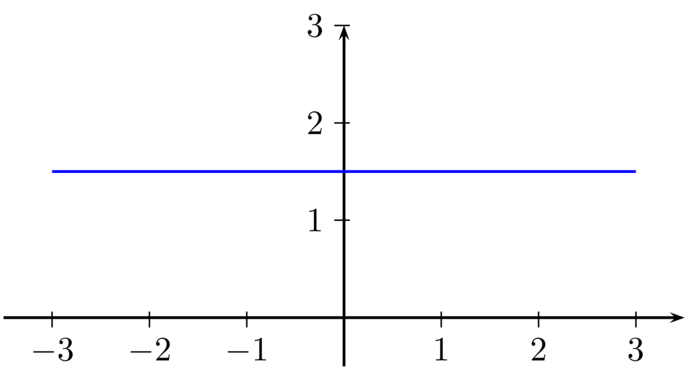
\includegraphics{Picture_FIGLabelFigFoncConstFdDkhWPICTFoncConstFdDkhW-for_eps.pdf}
%The result is on figure \ref{LabelFigFoncConstFdDkhW}.
%\newcommand{\CaptionFigFoncConstFdDkhW}{<+Type your caption here+>}
\input{Fig_FoncConstFdDkhW.pstricks}

\end{multicols}


\subsection{Sens de variation d'une fonction affine}

\begin{Aretenir}
      Soit $f$ la fonction affine $x\mapsto ax+b$.
      \begin{itemize}
      \item Si $a>0$, alors $f$ est croissante sur $\eR$.
      \item Si $a<0$, alors $f$ est décroissante sur $\eR$.
      \item Si $a=0$, alors $f$ est constante sur $\eR$
        (et $f(x)=b$ pour tout $x\in\eR$).
      \end{itemize}
\end{Aretenir}
Nous savons que si \( f(x)=ax+b\), alors \( f\) s'annule en \( x=-\frac{ b }{ a }\). Cela nous sert à écrire un tableau de signe de \( f\).



Les figures \ref{LabelFigFnAffineipcEQfssLabelSubFigFnAffineipcEQf0} et \ref{LabelFigFnAffineipcEQfssLabelSubFigFnAffineipcEQf1} montrent des droites affines. Lorsque \( a>0\), la droite monte; lorsque \( a<0\) elle descend. La pente est d'autant plus forte que \( a\) est grand.
\newcommand{\CaptionFigFnAffineipcEQf}{Deux droites affines.}
\input{Fig_FnAffineipcEQf.pstricks}




\begin{Aretenir}
      Règle du signe de $ax+b$ \\
      
      \begin{tabular}{cc}
        $a<0$ & $a>0$ \\
        & \\
        $\begin{array}{|c|ccccc|}
          \hline
          x & -\infty & & -\dfrac{b}{a} & & +\infty \\[2ex]
          \hline
          ax+b & & + \quad \ & 0 & \quad - & \\[1ex]
          \hline
        \end{array}$
        &
        $\begin{array}{|c|ccccc|}
          \hline
          x & -\infty & & -\dfrac{b}{a} & & +\infty \\[2ex]
          \hline
          ax+b & & - \quad \ & 0 & \quad + & \\[1ex]
          \hline
        \end{array}$ \\
      \end{tabular}  \\[1ex] 
\end{Aretenir}

\subsection{Tableau de variations}

Le \defe{tableau de variation}{tableau de variation} est un tableau contenant
\begin{enumerate}
    \item
        les positions des sommets,
    \item
        les flèches indiquant les endroits où la fonction est croissante ou décroissante.
\end{enumerate}
Un petit exemple valant mieux qu'un long discours\ldots

\begin{multicols}{2}

    Le tableau de variation de la fonction dessinée ci-contre est :
    \begin{equation}
    \begin{array}[h]{|c|ccccccc|}
        \hline
        x&-3&&-2&&0&&2\\
        \hline
        &&&2&&&&1\\
        f(x)&&\nearrow&&\searrow&&\nearrow&\\
        &\frac{ 9 }{2}&&&&-\frac{ 1 }{2}&&\\
        \hline
    \end{array}
    \end{equation}
    En effet, la fonction \( f\)
    \begin{itemize}
        \item 
            part de \( x=-3\) où \( f(x)=-9/2\);
        \item
            elle monte jusqu'en \( x=-2\) où elle vaut \( f(x)=2\);
        \item
            elle descend jusqu'en \( x=0\) où elle vaut \( -\frac{ 1 }{2}\);
        \item
            elle monte jusqu'en \( x=2\) où elle vaut \( 1\).
    \end{itemize}

\columnbreak


%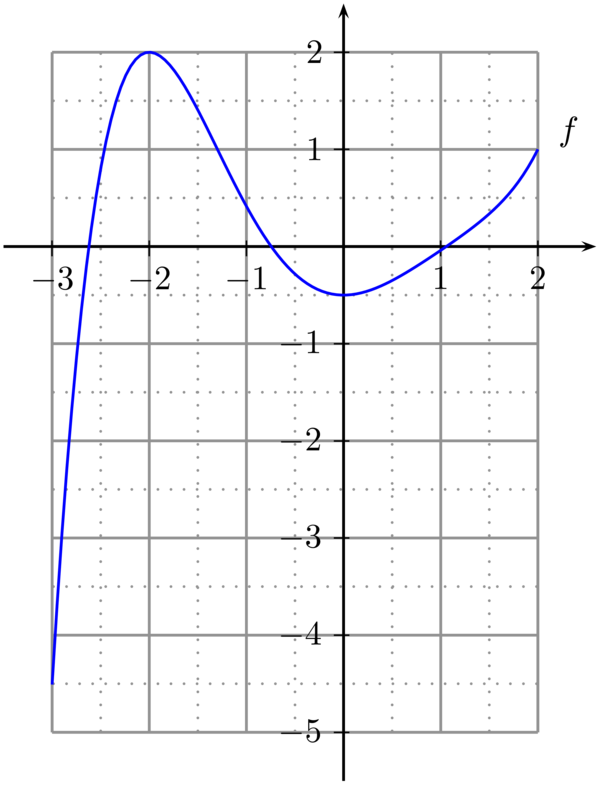
\includegraphics{Picture_FIGLabelFigGrapheVarREGMqxPICTGrapheVarREGMqx-for_eps.pdf}
%The result is on figure \ref{LabelFigGrapheVarREGMqx}.
%\newcommand{\CaptionFigGrapheVarREGMqx}{<+Type your caption here+>}
\input{Fig_GrapheVarREGMqx.pstricks}

\end{multicols}

\section{Minimum et maximum}

\begin{definition}
      Soit $f$ une fonction définie sur un intervalle $I$. \\[-2ex] 
      \begin{itemize}
          \item On dit que $f$ admet le réel $m$ pour \defe{minimum}{minimum (d'une fonction)}
        sur $I$ si et seulement si il existe $c\in I$ tel que $f(c)=m$
        et pour tout $x\in I$, $f(x)\geq m$. \\[-2ex]
    \item On dit que $f$ admet le réel $M$ pour \defe{maximum}{maximum}
        sur $I$ si et seulement si il existe $d\in I$ tel que $f(d)=M$ et pour tout
        $x\in I$, $f(x)\leq M$.
      \end{itemize}
\end{definition}

Sur la figure \ref{LabelFigMinMaxKNRdOd}, nous avons indiqué le minimum et le maximum de la fonction dessinée.
\newcommand{\CaptionFigMinMaxKNRdOd}{Minimum et maximum d'une fonction.}
\input{Fig_MinMaxKNRdOd.pstricks}


%+++++++++++++++++++++++++++++++++++++++++++++++++++++++++++++++++++++++++++++++++++++++++++++++++++++++++++++++++++++++++++
\section{Fonction carré}
%+++++++++++++++++++++++++++++++++++++++++++++++++++++++++++++++++++++++++++++++++++++++++++++++++++++++++++++++++++++++++++

<++>

%+++++++++++++++++++++++++++++++++++++++++++++++++++++++++++++++++++++++++++++++++++++++++++++++++++++++++++++++++++++++++++
\section{Fonction inverse}
%+++++++++++++++++++++++++++++++++++++++++++++++++++++++++++++++++++++++++++++++++++++++++++++++++++++++++++++++++++++++++++

<++>

%+++++++++++++++++++++++++++++++++++++++++++++++++++++++++++++++++++++++++++++++++++++++++++++++++++++++++++++++++++++++++++
\section{Exercices à propos des fonctions}
%+++++++++++++++++++++++++++++++++++++++++++++++++++++++++++++++++++++++++++++++++++++++++++++++++++++++++++++++++++++++++++

%---------------------------------------------------------------------------------------------------------------------------
\subsection{Image, antécédent}
%---------------------------------------------------------------------------------------------------------------------------

\Exo{Seconde-0042}
\Exo{Seconde-0048}
\Exo{Seconde-0054}
\Exo{Seconde-0051}
\Exo{Seconde-0050}

%---------------------------------------------------------------------------------------------------------------------------
\subsection{Exemples de fonctions}
%---------------------------------------------------------------------------------------------------------------------------

\Exo{Seconde-0058}
\Exo{Seconde-0057}
\Exo{Seconde-0063}
\Exo{Seconde-0061}
\Exo{Seconde-0067}

%---------------------------------------------------------------------------------------------------------------------------
\subsection{Représentation graphique}
%---------------------------------------------------------------------------------------------------------------------------

\Exo{Seconde-0043}
\Exo{Seconde-0059}
\Exo{Seconde-0047}
\Exo{Seconde-0060}
\Exo{Seconde-0049}

%---------------------------------------------------------------------------------------------------------------------------
\subsection{Travail sur les graphiques}
%---------------------------------------------------------------------------------------------------------------------------

\Exo{Seconde-0069}
\Exo{Seconde-0070}
\Exo{Seconde-0071}

%TODO : supprimer ce \newpage
\clearpage

\vspace{1cm}

\newpage        

% TODO : ce serait pas mal de mettre une question pleine de texte ici.

\Exo{smath-0015}
\Exo{Seconde-0072}

%---------------------------------------------------------------------------------------------------------------------------
\subsection{Équations linéaires et affines}
%---------------------------------------------------------------------------------------------------------------------------

\Exo{smath-0016}

%---------------------------------------------------------------------------------------------------------------------------
\subsection{Problèmes et résolution d'équation}
%---------------------------------------------------------------------------------------------------------------------------

\Exo{smath-0086}
\Exo{smath-0001}
\Exo{smath-0004}
\Exo{smath-0005}
\Exo{smath-0006}
\Exo{Seconde-0046}
\Exo{smath-0078}
\Exo{smath-0013}
\Exo{Seconde-0068}
\Exo{Seconde-0064}
\Exo{Seconde-0044}
\Exo{Seconde-0066}
\Exo{Seconde-0075}
\Exo{Seconde-0076}

%---------------------------------------------------------------------------------------------------------------------------
\subsection{Algorithmique}
%---------------------------------------------------------------------------------------------------------------------------

\Exo{smath-0002}
\Exo{smath-0003}
\Exo{Seconde-0086}
\Exo{smath-0007}
\Exo{smath-0008}

%---------------------------------------------------------------------------------------------------------------------------
\subsection{Plus avancés}
%---------------------------------------------------------------------------------------------------------------------------

\Exo{Premiere-0018}

%---------------------------------------------------------------------------------------------------------------------------
\subsection{Fonctions du second degré}
%---------------------------------------------------------------------------------------------------------------------------

\Exo{smath-0087}
\Exo{smath-0088}

